\documentclass{ximera}

%\usepackage{todonotes}

\newcommand{\todo}{}

\usepackage{esint} % for \oiint
\ifxake%%https://math.meta.stackexchange.com/questions/9973/how-do-you-render-a-closed-surface-double-integral
\renewcommand{\oiint}{{\large\bigcirc}\kern-1.56em\iint}
\fi


\graphicspath{
  {./}
  {ximeraTutorial/}
  {basicPhilosophy/}
  {functionsOfSeveralVariables/}
  {normalVectors/}
  {lagrangeMultipliers/}
  {vectorFields/}
  {greensTheorem/}
  {shapeOfThingsToCome/}
  {dotProducts/}
  {partialDerivativesAndTheGradientVector/}
  {../productAndQuotientRules/exercises/}
  {../normalVectors/exercisesParametricPlots/}
  {../continuityOfFunctionsOfSeveralVariables/exercises/}
  {../partialDerivativesAndTheGradientVector/exercises/}
  {../directionalDerivativeAndChainRule/exercises/}
  {../commonCoordinates/exercisesCylindricalCoordinates/}
  {../commonCoordinates/exercisesSphericalCoordinates/}
  {../greensTheorem/exercisesCurlAndLineIntegrals/}
  {../greensTheorem/exercisesDivergenceAndLineIntegrals/}
  {../shapeOfThingsToCome/exercisesDivergenceTheorem/}
  {../greensTheorem/}
  {../shapeOfThingsToCome/}
  {../separableDifferentialEquations/exercises/}
  {vectorFields/}
}

\newcommand{\mooculus}{\textsf{\textbf{MOOC}\textnormal{\textsf{ULUS}}}}

\usepackage{tkz-euclide}
\usepackage{tikz}
\usepackage{tikz-cd}
\usetikzlibrary{arrows}
\tikzset{>=stealth,commutative diagrams/.cd,
  arrow style=tikz,diagrams={>=stealth}} %% cool arrow head
\tikzset{shorten <>/.style={ shorten >=#1, shorten <=#1 } } %% allows shorter vectors

\usetikzlibrary{backgrounds} %% for boxes around graphs
\usetikzlibrary{shapes,positioning}  %% Clouds and stars
\usetikzlibrary{matrix} %% for matrix
\usepgfplotslibrary{polar} %% for polar plots
\usepgfplotslibrary{fillbetween} %% to shade area between curves in TikZ
%\usetkzobj{all}
\usepackage[makeroom]{cancel} %% for strike outs
%\usepackage{mathtools} %% for pretty underbrace % Breaks Ximera
%\usepackage{multicol}
\usepackage{pgffor} %% required for integral for loops



%% http://tex.stackexchange.com/questions/66490/drawing-a-tikz-arc-specifying-the-center
%% Draws beach ball
\tikzset{pics/carc/.style args={#1:#2:#3}{code={\draw[pic actions] (#1:#3) arc(#1:#2:#3);}}}



\usepackage{array}
\setlength{\extrarowheight}{+.1cm}
\newdimen\digitwidth
\settowidth\digitwidth{9}
\def\divrule#1#2{
\noalign{\moveright#1\digitwidth
\vbox{\hrule width#2\digitwidth}}}




% \newcommand{\RR}{\mathbb R}
% \newcommand{\R}{\mathbb R}
% \newcommand{\N}{\mathbb N}
% \newcommand{\Z}{\mathbb Z}

\newcommand{\sagemath}{\textsf{SageMath}}


%\renewcommand{\d}{\,d\!}
%\renewcommand{\d}{\mathop{}\!d}
%\newcommand{\dd}[2][]{\frac{\d #1}{\d #2}}
%\newcommand{\pp}[2][]{\frac{\partial #1}{\partial #2}}
% \renewcommand{\l}{\ell}
%\newcommand{\ddx}{\frac{d}{\d x}}

% \newcommand{\zeroOverZero}{\ensuremath{\boldsymbol{\tfrac{0}{0}}}}
%\newcommand{\inftyOverInfty}{\ensuremath{\boldsymbol{\tfrac{\infty}{\infty}}}}
%\newcommand{\zeroOverInfty}{\ensuremath{\boldsymbol{\tfrac{0}{\infty}}}}
%\newcommand{\zeroTimesInfty}{\ensuremath{\small\boldsymbol{0\cdot \infty}}}
%\newcommand{\inftyMinusInfty}{\ensuremath{\small\boldsymbol{\infty - \infty}}}
%\newcommand{\oneToInfty}{\ensuremath{\boldsymbol{1^\infty}}}
%\newcommand{\zeroToZero}{\ensuremath{\boldsymbol{0^0}}}
%\newcommand{\inftyToZero}{\ensuremath{\boldsymbol{\infty^0}}}



% \newcommand{\numOverZero}{\ensuremath{\boldsymbol{\tfrac{\#}{0}}}}
% \newcommand{\dfn}{\textbf}
% \newcommand{\unit}{\,\mathrm}
% \newcommand{\unit}{\mathop{}\!\mathrm}
% \newcommand{\eval}[1]{\bigg[ #1 \bigg]}
% \newcommand{\seq}[1]{\left( #1 \right)}
% \renewcommand{\epsilon}{\varepsilon}
% \renewcommand{\phi}{\varphi}


% \renewcommand{\iff}{\Leftrightarrow}

% \DeclareMathOperator{\arccot}{arccot}
% \DeclareMathOperator{\arcsec}{arcsec}
% \DeclareMathOperator{\arccsc}{arccsc}
% \DeclareMathOperator{\si}{Si}
% \DeclareMathOperator{\scal}{scal}
% \DeclareMathOperator{\sign}{sign}


%% \newcommand{\tightoverset}[2]{% for arrow vec
%%   \mathop{#2}\limits^{\vbox to -.5ex{\kern-0.75ex\hbox{$#1$}\vss}}}
% \newcommand{\arrowvec}[1]{{\overset{\rightharpoonup}{#1}}}
% \renewcommand{\vec}[1]{\arrowvec{\mathbf{#1}}}
% \renewcommand{\vec}[1]{{\overset{\boldsymbol{\rightharpoonup}}{\mathbf{#1}}}}

% \newcommand{\point}[1]{\left(#1\right)} %this allows \vector{ to be changed to \vector{ with a quick find and replace
% \newcommand{\pt}[1]{\mathbf{#1}} %this allows \vec{ to be changed to \vec{ with a quick find and replace
% \newcommand{\Lim}[2]{\lim_{\point{#1} \to \point{#2}}} %Bart, I changed this to point since I want to use it.  It runs through both of the exercise and exerciseE files in limits section, which is why it was in each document to start with.

% \DeclareMathOperator{\proj}{\mathbf{proj}}
% \newcommand{\veci}{{\boldsymbol{\hat{\imath}}}}
% \newcommand{\vecj}{{\boldsymbol{\hat{\jmath}}}}
% \newcommand{\veck}{{\boldsymbol{\hat{k}}}}
% \newcommand{\vecl}{\vec{\boldsymbol{\l}}}
% \newcommand{\uvec}[1]{\mathbf{\hat{#1}}}
% \newcommand{\utan}{\mathbf{\hat{t}}}
% \newcommand{\unormal}{\mathbf{\hat{n}}}
% \newcommand{\ubinormal}{\mathbf{\hat{b}}}

% \newcommand{\dotp}{\bullet}
% \newcommand{\cross}{\boldsymbol\times}
% \newcommand{\grad}{\boldsymbol\nabla}
% \newcommand{\divergence}{\grad\dotp}
% \newcommand{\curl}{\grad\cross}
%\DeclareMathOperator{\divergence}{divergence}
%\DeclareMathOperator{\curl}[1]{\grad\cross #1}
% \newcommand{\lto}{\mathop{\longrightarrow\,}\limits}

% \renewcommand{\bar}{\overline}

\colorlet{textColor}{black}
\colorlet{background}{white}
\colorlet{penColor}{blue!50!black} % Color of a curve in a plot
\colorlet{penColor2}{red!50!black}% Color of a curve in a plot
\colorlet{penColor3}{red!50!blue} % Color of a curve in a plot
\colorlet{penColor4}{green!50!black} % Color of a curve in a plot
\colorlet{penColor5}{orange!80!black} % Color of a curve in a plot
\colorlet{penColor6}{yellow!70!black} % Color of a curve in a plot
\colorlet{fill1}{penColor!20} % Color of fill in a plot
\colorlet{fill2}{penColor2!20} % Color of fill in a plot
\colorlet{fillp}{fill1} % Color of positive area
\colorlet{filln}{penColor2!20} % Color of negative area
\colorlet{fill3}{penColor3!20} % Fill
\colorlet{fill4}{penColor4!20} % Fill
\colorlet{fill5}{penColor5!20} % Fill
\colorlet{gridColor}{gray!50} % Color of grid in a plot

\newcommand{\surfaceColor}{violet}
\newcommand{\surfaceColorTwo}{redyellow}
\newcommand{\sliceColor}{greenyellow}




\pgfmathdeclarefunction{gauss}{2}{% gives gaussian
  \pgfmathparse{1/(#2*sqrt(2*pi))*exp(-((x-#1)^2)/(2*#2^2))}%
}


%%%%%%%%%%%%%
%% Vectors
%%%%%%%%%%%%%

%% Simple horiz vectors
\renewcommand{\vector}[1]{\left\langle #1\right\rangle}


%% %% Complex Horiz Vectors with angle brackets
%% \makeatletter
%% \renewcommand{\vector}[2][ , ]{\left\langle%
%%   \def\nextitem{\def\nextitem{#1}}%
%%   \@for \el:=#2\do{\nextitem\el}\right\rangle%
%% }
%% \makeatother

%% %% Vertical Vectors
%% \def\vector#1{\begin{bmatrix}\vecListA#1,,\end{bmatrix}}
%% \def\vecListA#1,{\if,#1,\else #1\cr \expandafter \vecListA \fi}

%%%%%%%%%%%%%
%% End of vectors
%%%%%%%%%%%%%

%\newcommand{\fullwidth}{}
%\newcommand{\normalwidth}{}



%% makes a snazzy t-chart for evaluating functions
%\newenvironment{tchart}{\rowcolors{2}{}{background!90!textColor}\array}{\endarray}

%%This is to help with formatting on future title pages.
\newenvironment{sectionOutcomes}{}{}



%% Flowchart stuff
%\tikzstyle{startstop} = [rectangle, rounded corners, minimum width=3cm, minimum height=1cm,text centered, draw=black]
%\tikzstyle{question} = [rectangle, minimum width=3cm, minimum height=1cm, text centered, draw=black]
%\tikzstyle{decision} = [trapezium, trapezium left angle=70, trapezium right angle=110, minimum width=3cm, minimum height=1cm, text centered, draw=black]
%\tikzstyle{question} = [rectangle, rounded corners, minimum width=3cm, minimum height=1cm,text centered, draw=black]
%\tikzstyle{process} = [rectangle, minimum width=3cm, minimum height=1cm, text centered, draw=black]
%\tikzstyle{decision} = [trapezium, trapezium left angle=70, trapezium right angle=110, minimum width=3cm, minimum height=1cm, text centered, draw=black]


\title{Systems}

\begin{document}

\begin{abstract}
intersection
\end{abstract}
\maketitle



\subsection*{Common Pairs}

Your journey through mathematics has brought you to a major change in your thinking. You have been working with individual numbers for years and years and years. Numbers have been the fundamental object in mathematics. Functions bring a totally different viewpoint. Our new basic mathematical tool is expanding from a number to a function.  Our new basic thought is about huge collections of pairs of numbers.  Our new analysis is moving from how numbers combine and compare to how functions combine and compare.

We are learning how to investigate functions.  Given a function, we would like to know its domain and range, zeros, discontinuities, singularities, where it is increasing or decreasing, what are the maximum and minum values, and what its graph looks like.

We would also like to compare functions.  For instance, what pairs functions might have in common. Let's try this for linear functions.



\subsection*{Intersections}

Given two linear functions, (1) do they share any pairs? (2) what are the common pairs?



If $f$ and $g$ are two linear functions and they shared the pair $(a, b)$, then we would have $f(a)=b$ and $g(a)=b$.  Their graphs would share a point. The lines would intersect. Since each linear function corresponds to exactly one line, it might be benefitial to think geometrically.  

How can two lines intersect?

\begin{example} One Point 

Two lines can interesect in exactly one point.
\begin{image}
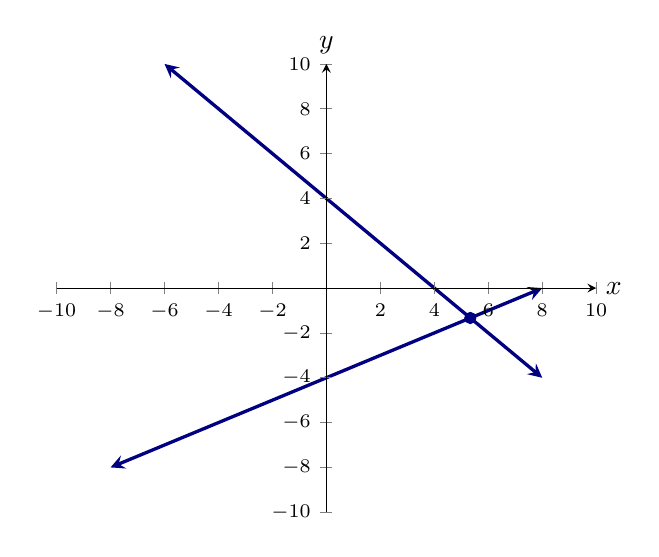
\begin{tikzpicture}
     \begin{axis}[
            	domain=-10:10, ymax=10, xmax=10, ymin=-10, xmin=-10,
            	axis lines =center, xlabel=$x$, ylabel=$y$, 
                ytick={-10,-8,-6,-4,-2,2,4,6,8,10}, 
                xtick={-10,-8,-6,-4,-2,2,4,6,8,10},
                ticklabel style={font=\scriptsize},
            	every axis y label/.style={at=(current axis.above origin),anchor=south},
            	every axis x label/.style={at=(current axis.right of origin),anchor=west},
            	axis on top,
          		]

        
        \addplot [draw=penColor, very thick, smooth, domain=(-8:8),<->] {0.5*x-4};
        \addplot [draw=penColor, very thick, smooth, domain=(-6:8),<->] {-x+4};
        \addplot[color=penColor,fill=penColor,only marks,mark=*] coordinates{(5.333,-1.333)};


    \end{axis}
\end{tikzpicture}
\end{image}


\end{example}

One point of intersection is probably the usual expectation.



The other two possibilities are more uncommon.









\begin{example} No Intersection 

Parallel lines would not intersect.
\begin{image}
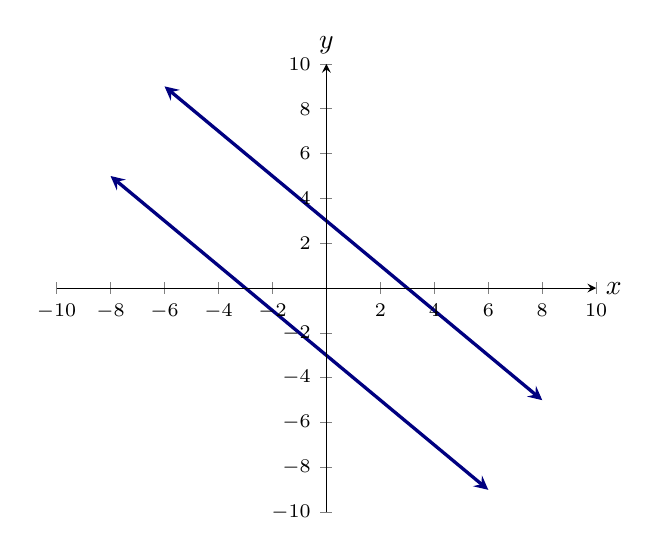
\begin{tikzpicture}
     \begin{axis}[
                domain=-10:10, ymax=10, xmax=10, ymin=-10, xmin=-10,
                axis lines =center, xlabel=$x$, ylabel=$y$,
                ytick={-10,-8,-6,-4,-2,2,4,6,8,10}, 
                xtick={-10,-8,-6,-4,-2,2,4,6,8,10},
                ticklabel style={font=\scriptsize},
                every axis y label/.style={at=(current axis.above origin),anchor=south},
                every axis x label/.style={at=(current axis.right of origin),anchor=west},
                axis on top,
                ]

        
        \addplot [draw=penColor, very thick, smooth, domain=(-8:6),<->] {-x-3};
        \addplot [draw=penColor, very thick, smooth, domain=(-6:8),<->] {-x+3};

        %\addplot[color=penColor2,fill=penColor,only marks,mark=*] coordinates{(16/3,-4/3)};
        %\addplot[color=penColor,fill=penColor,only marks,mark=*] coordinates{(6,-1)};


    \end{axis}
\end{tikzpicture}
\end{image}

Distinct linear functions with the same rate of chage cannot share any pairs.

\end{example}










\begin{example} Everywhere 

Two lines that were in fact the same line, would intersect at every point, because they are the same line.
\begin{image}
\begin{tikzpicture}
     \begin{axis}[
                domain=-10:10, ymax=10, xmax=10, ymin=-10, xmin=-10,
                axis lines =center, xlabel=$x$, ylabel=$y$,
                ytick={-10,-8,-6,-4,-2,2,4,6,8,10}, 
                xtick={-10,-8,-6,-4,-2,2,4,6,8,10},
                ticklabel style={font=\scriptsize},
                every axis y label/.style={at=(current axis.above origin),anchor=south},
                every axis x label/.style={at=(current axis.right of origin),anchor=west},
                axis on top,
                ]

        
        \addplot [draw=penColor, very thick, smooth, domain=(-8:8),<->] {x-1};


    \end{axis}
\end{tikzpicture}
\end{image}


While this is completely obvious when examining graphs, it might not be so obvious during an algebraic investigation.

It might not be immediate clear that $L(k) = \frac{4}{3}k - \frac{8}{5}$ and $p(h) = \frac{4(5h-6)}{15}$ are in fact the same linear function and share every pair.

\end{example}










\subsection*{Proof}



Linear functions can share no pairs, exactly $1$ pair, or all of their pairs.  Is that it?  Our intuition tells us that the graph of a line cannot turn around and have a second intersection point.  But, that is far from a convincing argument.  Perhaps the graphs do not show enough and our intuition is wrong.  

How do we convince people that this is true, without saying ``trust me''?

Graphing and Geometry are excellent tools for believing, but when you need an argument that accounts for \textbf{\textcolor{purple!85!blue}{EVERYTHING}}, then you need Algebra.  Algebra helps us make sure we have accounted for \textbf{\textcolor{purple!85!blue}{EVERYTHING}}.  



Reasoning that accounts for everything, is called \textbf{proof}.














\begin{explanation} Proof 


Let $f(x) = m_1 \, x + b_1$ and $g(x) = m_2 \, x + b_2$ be two linear functions with domains $(-\infty, \infty)$. \\
Suppose they share a pair. Let's call it $(T, R)$.

Then we have 

\begin{itemize}
\item $f(T) = m_1 T + b_1$
\item $g(T) = m_2 T + b_2$
\end{itemize}

If they share this pair, then $f(T) = g(T)$, which gives us

\[     m_1 \, T + b_1 =  m_2 \, T + b_2  \]


What are all of the possibilities?  For EVERY possibility, either $m_1 \ne m_2$ or $m_1 = m_2$.  These two ``cases'' account for EVERYTHING.


\textbf{case 1:}  $m_1 \ne m_2$ \\

If the rates of change are different, then  $m_1 - m_2 \ne 0$.  We can divide by $m_1 - m_2$, which allows us to solve for $T$.

\[     m_1 \, T - m_2 \, T =  b_2 -b_1 \]


\[     T =  \frac{b_2 -b_1}{m_1 - m_2}  \]

This fraction is valid since the denominator does not equal $0$.  Therefore, $T$ has one value.  $f$ and $g$ have exactly one pair in common.  The corresponding lines have one point of intersection.



\textbf{case 2:}  $m_1 = m_2$ \\



Setting $f(T) = g(T)$ gives us 



\[     m_1 \, T - m_1 \, T =  b_2 - b_1 \]


\[     0 \, T =  b_2 - b_1 \]


What values of $T$ make this true?


\begin{itemize}
\item If $b_2 \ne b_1$, then no value of $T$ will make the equation true.  We have parallel lines with no intersection.

\item If $b_2 = b_1$, then we have $0 \, T =  0$ and every value of $T$ will make the equation true.  In this case, we have $m_1 = m_2$ and $b_1 = b_2$.  We have the same function and the same line.
\end{itemize}



And, that is \textbf{\textcolor{purple!85!blue}{ALL}} of the possibilities.  $b_2 \ne b_1$ and  $b_2 = b_1$ account for every possiblity.  The two statements together constitute a proof.


\begin{itemize}
\item Two linear functions have one pair in common. Their lines have exactly one intersection point, or

\item Two linear functions share no pairs and their lines are parallel, or

\item Two linear functions are the same function and have the same line.



\end{itemize}





\end{explanation}


As a consequence, if you know you have two linear functions and you know they share two points, then they must share all of their points and they must be the same function.   

This is why we only need two points to draw a line.
















\subsection*{Systems of Linear Equations}

The thinking above is part of a larger idea.


While we are currently considering two variables, a general linear equation can have any number of variables.


\[
a_n \, x_n + a_{n-1} \, x_{n-1} + \cdots + a_2 \, x_2 + a_1 \, x_1 + a_0 = 0
\]


We might collect some linear equations and group them together. This collection is called a \textbf{system of linear equations}. And, as above, we might look for common solutions.  The process of looking for common solutions is called \textit{solving the system}.





Systems are commonly written together with the equal signs aligned.

For example, the system might include two equations with two variables.

\begin{align*}
2x & = 3y + 5 \\
4x & = 7y + 11
\end{align*}



For example, the system might include two equations with three variables.

\begin{align*}
2x & = 3y - 3z + 5 \\
4x & = 7y - z - 7
\end{align*}




For example, the system might include three equations with three variables.

\begin{align*}
2x & = 3y - 3z + 5 \\
4x & = 7y - z - 7 \\
x & = y - z + 2 
\end{align*}


Or, some other combination. A system of linear equations can group any number of linear equations with any number of variables.  The study of these types of systems is called \textbf{Linear Algebra}.

For us, solving the system - identifying the common solutions - always uses the same thinking - \textbf{\textcolor{purple!85!blue}{EQUALITY}}.



\begin{fact} \textbf{\textcolor{purple!85!blue}{Replacement}} 

You can replace equal things with equal things and get equal things.

\end{fact}


\begin{fact} \textbf{\textcolor{purple!85!blue}{Operations}} 

You can do the same thing to equal things and get equal things.

\end{fact}






\begin{example} Solving a System


Solve the system
\begin{align*}
2x & = 3y + 5 \\
4x & = 7y + 11
\end{align*}



\begin{explanation}

Solving means to find a common pair of numbers that satisfy both equations or a common point on the graph. \\

Let's call this common pair or point $(x, y) = (A, B)$ \\

\begin{align*}
2A & = 3B + 5 \\
4A & = 7B + 11
\end{align*}



Then we have $2A = 3B + 5$. We can multiply both sides by $\answer{2}$ to get $4A = 6B + 10$.  \\

$2A = 3B + 5$ and $4A = 6B + 10$ are equivalent equations. \\

Therefore, we can replace the first equation in our system with this new equivalent equation.\\



\begin{align*}
4A & = 6B + 10 \\
4A & = 7B + 11
\end{align*}


We now have two expressions both equal to $4A$, then they must, themselves, be equal.


\[   6B + 10 =  \answer{7B + 11}   \]

We can subtract $6B$ from both sides and subtract $\answer{11}$ from both sides to get


\[   -1 =  B   \]



We now know that $B = -1$ and we know that $4A = 7B + 11$.  That tell us that 


\[   4A = 7(-1) + 11   \]

\[   4A = 4   \]


\[ A = 1 \]


Our common solution to the two original equations is $A = 1$ and $B = -1$.  If you graph the two lines, then $(1, -1)$ would be the intersection point.

\end{explanation}
\end{example}












\begin{example} Solving a System


Solve the system
\begin{align*}
x & = 3y - 1 \\
4x & = 5y + 3
\end{align*}

\begin{explanation}


Supposed $(x, y) = (A, B)$ is a solution.


\begin{align*}
A & = 3B - 1 \\
4A & = 5B + 3
\end{align*}


We have $A = 3B - 1$, therefore we can replace any $A$ with $\answer{3B - 1}$.  

\begin{align*}
A & = 3B - 1 \\
4(3B - 1) & = 5B + 3
\end{align*}


The second equation tells us that 


\[   4(3B - 1) = 5B + 3   \]

\[   12B - 4 = 5B + 3   \]


\[ 7B = 7 \]


\[ B = 1 \]

With this new information, the first equation in the system tells us that

\[ A = 3B - 1 \]

\[ A = 3(1) - 1 \]

\[ A = 2 \]

Our common solution to the two original equations is $A = 2$ and $B = 1$.  If you graph the two corresponding lines, then $(2, 1)$ would be the intersection point.

\end{explanation}
\end{example}









\begin{center}
\textbf{\textcolor{green!50!black}{ooooo-=-=-=-ooOoo-=-=-=-ooooo}} \\

more examples can be found by following this link\\ \link[More Examples of Linear Functions]{https://ximera.osu.edu/csccmathematics/precalculus1/precalculus1/linearFunctions/examples/exampleList}

\end{center}






\end{document}
